\documentclass[a4paper]{article}

\usepackage[T1]{fontenc}
\usepackage{graphicx}
\usepackage{amsmath}
\usepackage[utf8]{inputenc}
\usepackage{enumitem}
\setlist[description]{style=unboxed}

\usepackage{tikz}
\usepackage{pgfplots}
\usepackage{circuitikz}
\usepackage{tabularx}
\usepackage{rotating}
\usepackage{caption} 
\captionsetup[table]{skip=10pt}

\usetikzlibrary{calc,positioning,shapes,decorations.pathreplacing}

\tikzset{
	short/.style={draw,rectangle,text height=3pt,text depth=13pt,
		text width=7pt,align=center,fill=gray!30},
	long/.style={short,text width=1.5cm},
	verylong/.style={short,text width=4.5cm}
}

\begin{document}
\section{DC voltage power supply}

\subsection{Introduction}

For fully functional operation, submarine is equipped with 
lot of computer based subsystems and electronic devices which operate on DC 
voltage. To ensure their proper operation the, DC voltage has to be stable and 
without noise. To ensure stable DC voltage, device on Fig. 
\ref{fig:schematic}. is used. Device is composed of several parts as it is 
shown on the figure. Due to extreme conditions in the system, regulators often 
fail and components have to be repaired or replaced with proper spare part.

In this task, your job is to:
\begin{itemize}
\item find the parts which ensure proper operation of regulator, 
\item ensure that the output voltage ripple is within the boundaries with 
proper choice of parts for the low pass filter,
\item find the probability of future malfunction in standby redundant system.
\end{itemize}

\textbf{Device specifications.} Device specifications are provided with 
the following table. In each task you have to ensure that the values specified
in the table correspond to the values which will be measured in simulation. 

\begin{table}[h!]
    \hyphenpenalty 10000
    \caption{Device specifications}
    \label{tab:spec}
    \begin{tabularx}{\linewidth}{|X|X|X|X|} \hline
    PARAMETER & TEST CONDITIONS & VALUE & UNIT \\ \hline
    Input voltage ($U_{in}$)&  & $330$ & Vpp \\ \hline 
    Output voltage ($U_{out}$)& $I_{out} = 1$ A & $10$ ($\pm5$) \% & V \\ \hline
    Output current ($I_{out}$) & $U_{in} = 330$ Vpp & $1.0$ & A \\ \hline
    Ripple rejection & (12.8 kHz) & $78$ & dB \\ \hline
    \end{tabularx}
\end{table}

\begin{table}[h!]
    \hyphenpenalty 10000
    \caption{Device element values}
    \label{tab:elems}
    \begin{tabularx}{\linewidth}{|X|X|X|X|} \hline
    ELEMENT & PARAMETER & VALUE & UNIT \\ \hline
    $T_1$ & transfer ratio ($n$) & $25$ &  dimensionless \\ \hline
    $D_1$ & $U_{pn}$ & $0.6$ & V \\ \hline 
    $R_2$ & Resistance & $1$ & M$\Omega$ \\ \hline
    $R_4$ & Resistance & $470$ & k$\Omega$ \\ \hline
    $R_L$ & Resistance & 10 & $\Omega$ \\ \hline
    $Q_1$ & $U_{pn}$ & $0.6$ & V \\ \hline
    $C_1$ & Capacitance & $10$ & mF \\ \hline
    \end{tabularx}
\end{table}

\newpage

\subsection{Finding the proper choice of components}
\label{ele:task:1}
As it can be seen from the table \ref{tab:elems}, some components are not 
determined. In this subtask you need to specify resistor $R_1$ and diode $D_2$. 
Additionally, you have to determine positions of the negative and the positive 
input of the amplifier $A_1$. Based on the regulators operating values 
provided with table \ref{tab:spec} you have to determine specifications for 
the resistor $R_1$ and diode $D_2$. You have to find the components from the 
DigiKey Electronics product database. 

There are, however, constraints for your choice of components:
\begin{itemize}
\item $R_1$ has footprint given with figure Fig. \ref{fig:footprint},
\item $D_2$ is a through-hole component.
\end{itemize} 
 
Your choice is graded in several ways:
\begin{itemize}
\item component price,
\item correct component voltage, power and current ratings,
\item correct component footprint.
\end{itemize}
As a result, you have to provide two DigiKey part numbers for resistor and 
diode, respectively.

\begin{figure}[h!]
\centering
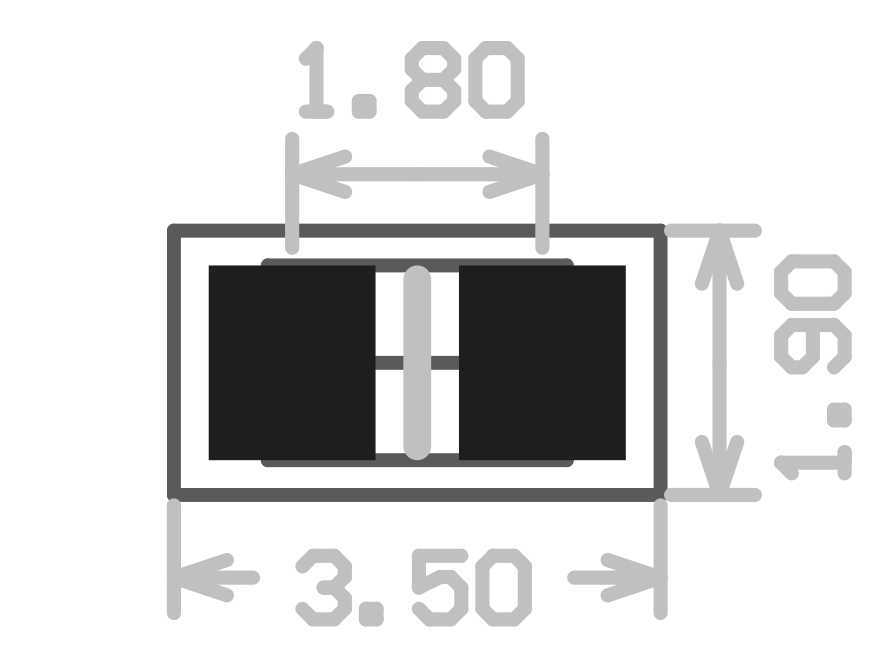
\includegraphics[width=\linewidth]{images/footprint.png}
\caption{Component footprint with dimension in millimeters}
\label{fig:footprint}
\end{figure}

\newpage

\subsection{LC filter design}
\label{ele:task:2}
To achieve specified ripple rejection at required frequency, design a LC low 
pass filter which filters output of a regulator. As in previous task you have 
to provide DigiKey part numbers for LC filter. \textbf{Note:} The ripple 
rejection of the regulator part of the device is $58$ dB at $12.8$ kHz.

Again, there are constraints for your choice of components:
\begin{itemize}
\item $L_1$ has no additional constraints 
(think about already mentioned implicit constraints),
\item $C_2$ has footprint given with Fig. \ref{fig:footprint},
\item $Q$ factor has to be equal $\frac{\sqrt{2}}{2}$ for $R_L = 10$ $\Omega$.  
\end{itemize}

Your choice is graded in the similar fashion as before:
\begin{itemize}
\item price,
\item correct inductance and capacitance,
\item correct footprints, 
\item correct current and voltage ratings.
\end{itemize}
As a result, you have to provide two DigiKey part numbers for inductor and 
capacitor, respectively. 
\newpage
\subsection{Side task: Reliability of the system with redundant power supply} 
\label{ele:task:3}
To increase reliability of the power supply system two different linear 
regulators are linked in configuration which is given with the Fig. 
\ref{fig:psc}. This configuration is known as passive standby redundancy. 
Probability of a failure in one regulator is modeled with exponential 
probability density function. More precisely, probability density function for 
the first regulator is:  
\begin{equation}
f_1(t) = \lambda_1 e^{-\lambda_1 t}
\end{equation}
and for the second regulator:
\begin{equation}
f_2(t) = \lambda_2 e^{-\lambda_2 t}
\end{equation}

Your task is to determine probability density function $f_S(t)$ which gives the
probability of failure in system described with Fig. \ref{fig:psc}. As a result 
provide probability of a failure for $t = 10000$ $h$ with:
\begin{itemize}
\item[] $\lambda_1 = 1 \cdot10^{-6}$ $h^{-1}$
\item[] $\lambda_2 = 2 \cdot10^{-6}$ $h^{-1}$ 
\end{itemize} 

\textbf{Note}: mean time between failures is increased $T_{sf} = 
T_{1f} + T_{2f}$. 

\begin{figure}[h!]
\centering
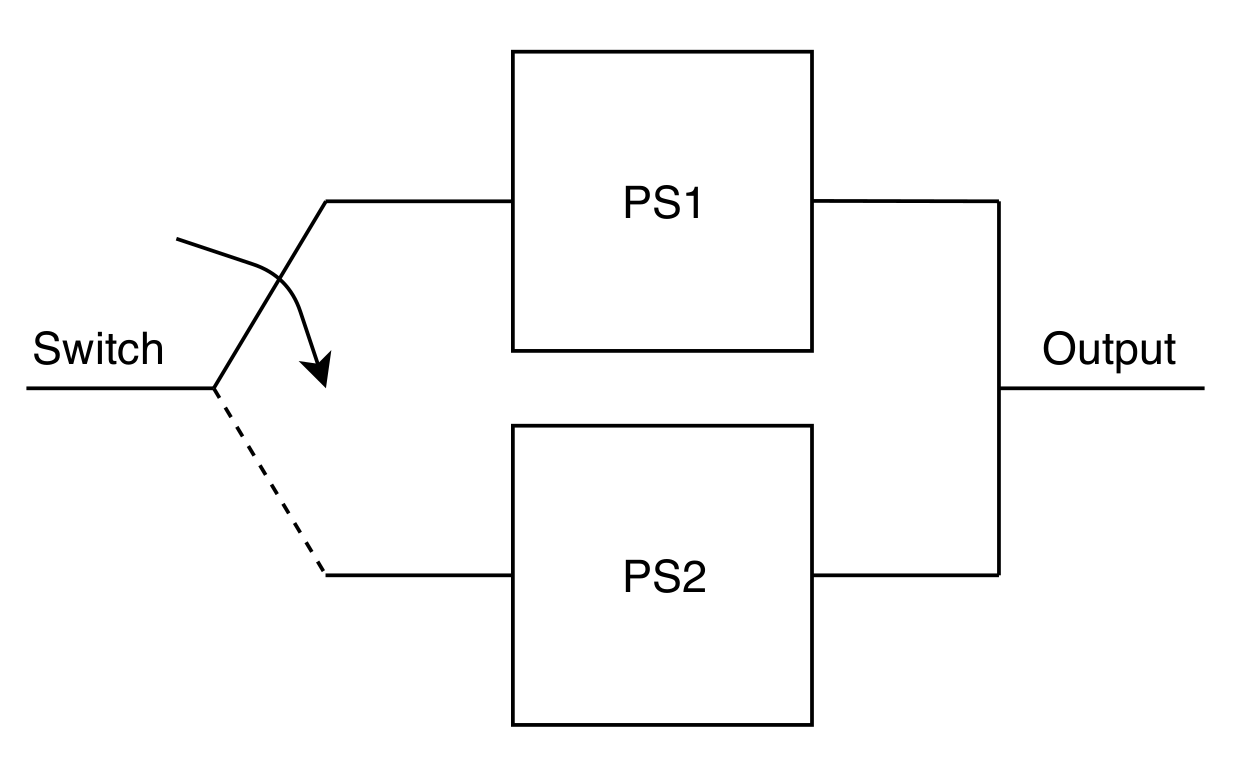
\includegraphics[width=\linewidth]{images/standby.png}
\caption{Standby system configuration}
\label{fig:psc}
\end{figure}

\newpage

\subsection{Solution format}
Solution for each task is a plain text document containing requested data. For
the tasks \ref{ele:task:1} and \ref{ele:task:2} text documents need to have 
two rows. One component part number in each row. Only one row is needed for the 
task \ref{ele:task:3} (requested probability). Name the files 
\texttt{task1.txt}, \texttt{task2.txt}, \texttt{task3.txt} and put them in 
the appropriate Google Drive folder.

Additionally, for the task \ref{ele:task:3} you have to provide documentation
which has to contain derivation of $f_S(t)$.

\subsection{Grading scheme}
Tasks are graded in the following manner:
\begin{itemize}
\item tasks \ref{ele:task:1} and \ref{ele:task:2} - up to \textbf{10 pts}, 
up to \textbf{5 pts} for each component.
\item task \ref{ele:task:3} - up to \textbf{10 pts} - \textbf{5 pts} for the 
correct probability and up to \textbf{5 pts} for correct documentation.
\end{itemize}

\begin{sidewaysfigure}[h!]
\centering
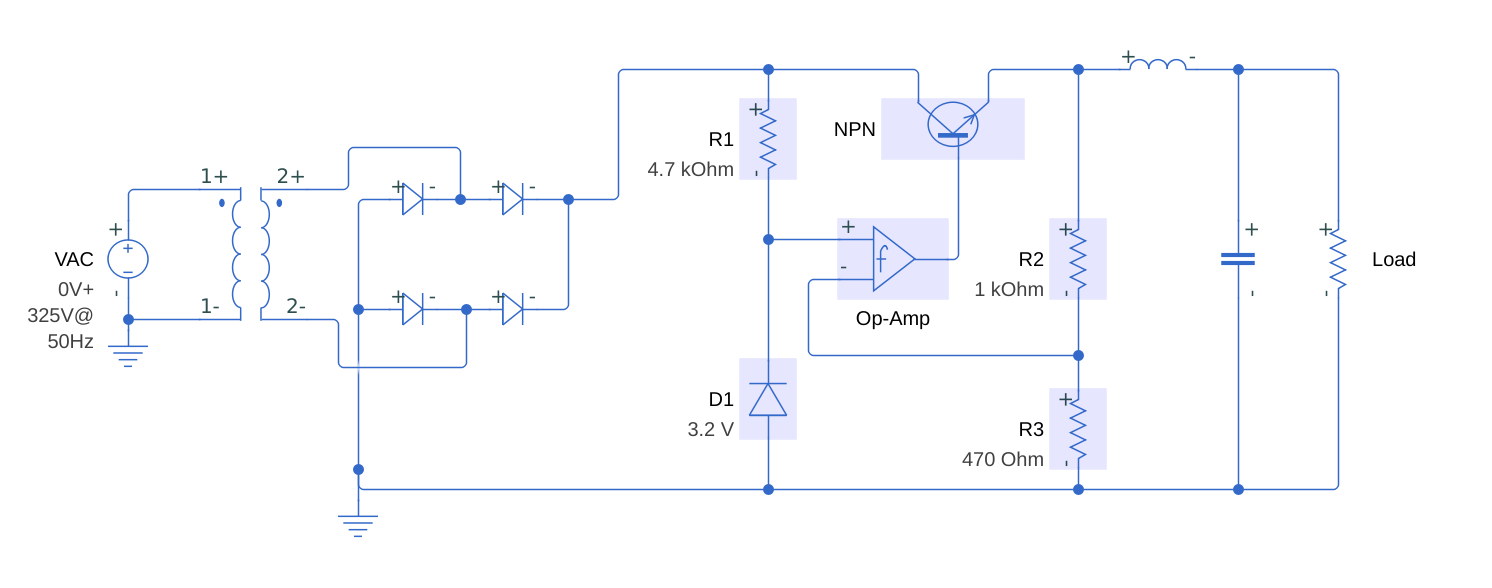
\includegraphics[width=\linewidth]{images/reg.png}
\caption{DC voltage power supply schematic}
\label{fig:schematic}
\end{sidewaysfigure}
 
\end{document}